\chapter{Описание стенда и подготовка}
\label{ch:stand}

\section{Конфигурация виртуального стенда}

Виртуальная машина \texttt{seafile} --- Ubuntu~22.04~LTS (VirtualBox),
один сетевой адаптер:
\begin{itemize}
  \item \textbf{Адаптер~1} (\texttt{enp0s3}) --- тип \textit{Internal Network
        (intnet)}: LAN-сегмент, статический IP \texttt{192.168.\cfgLabStudentN.4/24},
        шлюз \texttt{192.168.\cfgLabStudentN.1} (gateway), DNS \texttt{192.168.\cfgLabStudentN.1}.
\end{itemize}

% --- Скриншот: настройки ВМ seafile в VirtualBox (Сеть) ---
\begin{figure}[h]
  \centering
  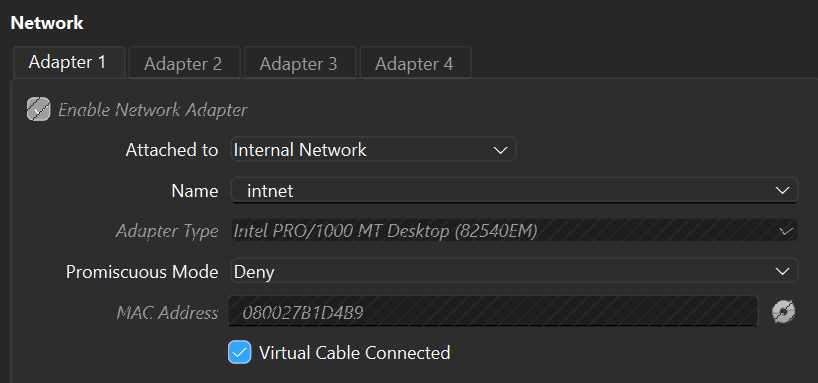
\includegraphics[width=0.85\textwidth]{img/01_vbox_seafile_settings}
  \caption{Настройки ВМ seafile --- адаптер Internal Network в VirtualBox}
  \label{fig:vbox_seafile}
\end{figure}

\section{Назначение статического IP (netplan)}

Поднимаем права до root:
\begin{lstlisting}
sudo su
\end{lstlisting}

Редактируем файл netplan:
\begin{lstlisting}
nano /etc/netplan/00-installer-config.yaml
\end{lstlisting}

Содержимое файла:
\begin{lstlisting}
network:
  ethernets:
    enp0s3:
      dhcp4: no
      addresses:
        - 192.168.N.4/24
      gateway4: 192.168.N.1
      nameservers:
        addresses: [192.168.N.1]
        search: [STUDENT.GROUP.local]
  version: 2
\end{lstlisting}

Применяем конфигурацию:
\begin{lstlisting}
netplan apply
\end{lstlisting}

Проверяем связь:
\begin{lstlisting}
ping gateway
ping ya.ru
\end{lstlisting}

% --- Скриншот: nano /etc/netplan/00-installer-config.yaml ---
\begin{figure}[h]
  \centering
  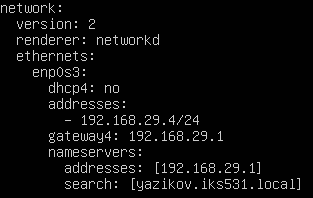
\includegraphics[width=0.85\textwidth]{img/02_netplan_seafile}
  \caption{Файл \texttt{netplan} ВМ seafile --- статический IP}
  \label{fig:netplan_seafile}
\end{figure}

% --- Скриншот: ping gateway и ping ya.ru ---
\begin{figure}[h]
  \centering
  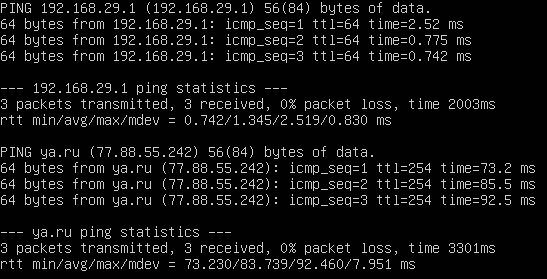
\includegraphics[width=0.85\textwidth]{img/03_ping_gateway}
  \caption{Проверка связи: \texttt{ping gateway} и \texttt{ping ya.ru}}
  \label{fig:ping_gw}
\end{figure}

\section{Переименование хоста}

\begin{lstlisting}
hostnamectl set-hostname seafile
nano /etc/hosts
\end{lstlisting}

В \texttt{/etc/hosts} привести строку к виду:
\begin{lstlisting}
127.0.0.1  localhost
127.0.1.1  seafile
\end{lstlisting}

Перезагружаем сервер:
\begin{lstlisting}
reboot
\end{lstlisting}

\section{Регистрация в DNS}

Подключаемся к ВМ \texttt{gateway} и добавляем A-запись в прямую зону.

\begin{lstlisting}
nano /var/lib/bind/forward.db
\end{lstlisting}

Добавляем строку в конце файла:
\begin{lstlisting}
seafile  IN  A  192.168.N.4
\end{lstlisting}

Перезапускаем BIND9:
\begin{lstlisting}
systemctl restart bind9
\end{lstlisting}

Проверяем:
\begin{lstlisting}
nslookup seafile
\end{lstlisting}

% --- Скриншот: nslookup seafile ---
\begin{figure}[h]
  \centering
  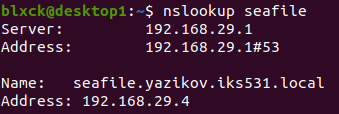
\includegraphics[width=0.85\textwidth]{img/04_nslookup_seafile}
  \caption{Разрешение имени \texttt{seafile} через DNS}
  \label{fig:nslookup_seafile}
\end{figure}

\endinput
